% !TeX program = pdflatex
% !TeX encoding = UTF-8
%=======================================================================
%  GRIS-NOT-001  ·  Plantilla de notas rápidas para la memoria
%  Proyecto 00503 - Generator inspection robotic system · Mecanalisis
%  Identidad: GRIS-IDENTIDAD-001 v1.4
%-----------------------------------------------------------------------
%  CÓMO USARLA (en 3 pasos)
%
%   1. Copiá este archivo con el código de la nota, en su propia carpeta:
%         memoria/notas/02489-00-MC007/02489-00-MC007.tex
%      El número (###) es correlativo: mirá la última nota y sumá uno.
%      Las figuras van en memoria/notas/02489-00-MC007/figuras/ y el PDF
%      final se copia a memoria/pdf/.
%
%   2. Completá los cuatro datos del bloque «DATOS DE LA NOTA».
%
%   3. Escribí:
%        · Resultados (obligatorio, siempre primero): lo que se sabe
%          ahora que antes no se sabía. Frases cortas, con números.
%        · El resto es libre. Usá los títulos que te sirvan, o ninguno.
%
%   Compilar desde la carpeta de la nota:  pdflatex 02489-00-MC007.tex
%   En Overleaf: subí el .tex y logo-gris.pdf.
%
%  LOGO: se usa «logo-gris.pdf» (GRIS-LOGO-003, reducido) de esta carpeta
%  o de ../../plantilla/. Si falta, se escribe «GRIS» como marcador.
%=======================================================================
\documentclass[11pt,a4paper]{article}

%=======================================================================
%  DATOS DE LA NOTA  ← lo único que hay que tocar arriba
%=======================================================================
\newcommand{\codigo}{02489-00-MC010}          % 02489-00-MC###
\newcommand{\titulo}{Evaluación de la cámara NanEyeC}
\newcommand{\autor}{Matías Gaviño}
\newcommand{\fecha}{01/10/2026}                    % o p. ej. {24/09/2026}

%=======================================================================
%  ESTILO  (no hace falta tocar nada de aquí hasta \begin{document})
%=======================================================================
\usepackage[T1]{fontenc}
\usepackage[utf8]{inputenc}
\usepackage[spanish,es-noshorthands,es-tabla]{babel}
\usepackage{lmodern}
\usepackage[a4paper,top=3.0cm,bottom=2.4cm,left=2.4cm,right=2.4cm,
            headheight=20pt,headsep=1.2cm,footskip=1.1cm]{geometry}
\usepackage{microtype}
\usepackage{xcolor}
\usepackage{graphicx}
\usepackage{booktabs}
\usepackage{array}
\usepackage{enumitem}
\usepackage{titlesec}
\usepackage{fancyhdr}
\usepackage{caption}
\usepackage{amsmath,amssymb}
\usepackage{float}
\usepackage{tabularx}
\usepackage[hidelinks]{hyperref}
\usepackage{xurl}

% --- colores -----------------------------------------------------------
\definecolor{gris-naranja}{HTML}{FF7A00}   % naranja institucional
\definecolor{tinta}{HTML}{1E2328}
\definecolor{gris-medio}{HTML}{6B7280}
\definecolor{gris-linea}{HTML}{DADDE1}
\color{tinta}

\hypersetup{pdftitle={\codigo\ -- \titulo}, pdfauthor={\autor},
            colorlinks=true, linkcolor=tinta, urlcolor=tinta}

% --- logo ---------------------------------------------------------------
\graphicspath{{./}{figuras/}{../../plantilla/}}
\newcommand{\logogris}{%
  \IfFileExists{logo-gris.pdf}
    {
\includegraphics[height=16pt]{logo-gris.pdf}}
    {\IfFileExists{../../plantilla/logo-gris.pdf}
      {
\includegraphics[height=16pt]{../../plantilla/logo-gris.pdf}}
      {{\fontsize{18}{18}\selectfont\bfseries\sffamily\color{gris-naranja}GRIS}}}}

% --- tipografía del cliente (código documental) --------------------------
% Geogrotesque no es libre; se usa Roboto Condensed Bold, que viene con
% TeX Live y Overleaf y tiene el mismo aire que el logo.
\newcommand{\fuentecliente}{\fontfamily{Roboto-TLF}\fontseries{bc}\selectfont}

% --- encabezado y pie ---------------------------------------------------
\pagestyle{fancy}
\fancyhf{}
\renewcommand{\headrulewidth}{0.4pt}
\renewcommand{\headrule}{\vspace{3pt}{\color{gris-linea}\hrule height \headrulewidth}}
\fancyhead[L]{\logogris}
\fancyhead[R]{{\fuentecliente\fontsize{12}{12}\selectfont\color{gris-medio}\codigo}}
\fancyfoot[R]{\footnotesize\color{gris-medio}\thepage}

% --- títulos numerados ----------------------------------------------------
\setcounter{secnumdepth}{2}
\titleformat{\section}{\large\bfseries}{\thesection}{0.8em}{}
\titleformat{\subsection}{\normalsize\bfseries}{\thesubsection}{0.8em}{}
\titlespacing*{\section}{0pt}{16pt}{5pt}
\titlespacing*{\subsection}{0pt}{11pt}{3pt}

% --- texto ------------------------------------------------------------------
\setlength{\parindent}{0pt}
\setlength{\parskip}{6pt}
\linespread{1.05}
\setlist{topsep=2pt, itemsep=2pt, parsep=0pt, leftmargin=1.2em}
\setlist[itemize]{label={\raisebox{0.15ex}{\small$\bullet$}}}
\captionsetup{font={small,color=gris-medio}, labelfont=bf, skip=5pt}
\renewcommand{\arraystretch}{1.25}

% --- cabecera de la nota ------------------------------------------------------
\newcommand{\cabecera}{%
  \thispagestyle{fancy}%
  {\fontsize{20}{24}\selectfont\bfseries\titulo\par}%
  \vspace{5pt}%
  {\small\color{gris-medio}\fecha\quad·\quad\autor\par}%
  \vspace{6pt}}

% --- ayudas opcionales --------------------------------------------------------
% \figura{archivo}{ancho}{pie}
\newcommand{\figura}[3]{%
  \begin{figure}[htbp]\centering
    \includegraphics[width=#2\linewidth]{#1}\caption{#3}
  \end{figure}}

%=======================================================================
\newcommand{\fig}[3]{%
  \begin{figure}[H]\centering
    \includegraphics[width=#2\linewidth]{#1}\caption{#3}
  \end{figure}}

\begin{document}
\cabecera

%=======================================================================
\section{Resultados}

\begin{itemize}
  \item \textbf{La ams OSRAM NanEyeC RGB es la única candidata relevada que cumple a la vez foco, color y montaje compacto.}
  Profundidad de campo publicada de 4~mm a infinito, 320\,$\times$\,320~px en color y cuerpo SGA de 1,04\,$\times$\,1,04\,$\times$\,2,29~mm con 4 pads soldables, sin cable~[S1].
  \item \textbf{Se conecta directo a la Kria K24 en modo SEIM con 2 pines del banco HDIO~26 (3,3~V).}
  La FPGA entrega el reloj (60--75~MHz) por SCLK y el sensor devuelve los datos por SDAT. A 75~MHz el cuadro dura 17,1~ms (58,5~cuadros/s) y el caudal útil es de 59,4~Mbit/s~[S1,~S5].
  \item \textbf{Densidad nominal de 26~px/mm a 5~mm, 16~px/mm a 8~mm y 11~px/mm a 12~mm} (campo de 12, 20 y 29~mm de ancho).
  Con la NanEyeM, que tiene la misma óptica, se midieron 11,2~mm de campo a 4~mm y 14,2~mm a 6~mm~[S7].
  \item \textbf{La nitidez es pareja entre 4 y 10~mm.}
  En la NanEyeM, el MTF50 vale 97 a 106~lp/mm en el plano del sensor entre 4 y 10~mm, y cae a 51~lp/mm a 2~mm~[S7].
  \item \textbf{No existe ninguna imagen pública de una NanEyeC de fábrica fotografiando texto o códigos a 5--12~mm.}
  Las más cercanas a ese caso son tres:
  \begin{itemize}
    \item una NanEye 2D viendo una carta USAF a 5 y 10~mm, detrás de una ventana propia del prototipo~[S9];
    \item una NanEye RGB de fábrica a 8~mm sobre relieves de 1~mm~[S8];
    \item una captura cruda de texto impreso con una NanEye 2C, a distancia no indicada~[S10].
  \end{itemize}
  \item \textbf{Lo que muestran las imágenes reales:} buen detalle en el centro, caída fuerte de luz y viñeteo hacia los bordes, reflejos especulares y distorsión de barril. La hoja de datos da $-15$\,\% en el borde del campo~[S1]. \textbf{La iluminación va a pesar tanto como la óptica.}
  \item \textbf{El suministro es el riesgo principal.}
  \begin{itemize}
    \item Hay un único fabricante y la versión RGB figura en \emph{preproducción}~[S3].
    \item Se vende solo por bandeja de 496~u: DigiKey, USD~58,443 c/u, 0 en stock, 12~semanas~[S4].
    \item El código viejo figura obsoleto porque la producción pasó a Focuslight con códigos nuevos; no es una discontinuación~[S2].
  \end{itemize}
  \item \textbf{La NanEye2D queda descartada.}
  \begin{itemize}
    \item La versión soldable (SGA) solo existe en blanco y negro, sin lente y con mínimo de 400~u.
    \item La RGB solo se vende con cable de 2~m.
    \item Su LVDS de 60~mV necesita un comparador externo~[S26].
  \end{itemize}
  \item \textbf{Siguiente paso:}
  \begin{itemize}
    \item comprar el kit NanoBerry color (DigiKey 14~u a USD~583,90; Mouser EU 3~u a EUR~450, al 01/10/2026);
    \item medir MTF, USAF, texto y códigos a 5, 8 y 12~mm con la iluminación real (sección~\ref{sec:prueba});
    \item pedirle a ams muestras del Q65113A9012 y la fecha de producción plena.
  \end{itemize}
\end{itemize}

%=======================================================================
\section{Contexto y requisitos}

GRIS necesita una cámara para ver objetos pequeños de muy cerca. Tiene que ir montada en el \emph{carrier} del robot, sin cables, y conectarse a la Kria K24 que ya lleva esa placa.

Se partió de una planilla de 32 alternativas (\emph{Alternativas\_camaras\_robot\_GRIS}, rev.~9, al 01/10/2026). Se filtró por foco publicado en 5--12~mm y luego por montaje sin cable. Pasaron ese filtro la NanEyeC, la NanEye2D en SGA, la OMNIVISION OCHTA10 y la OVM6946, y los cubos MiiS MCCA.
\begin{itemize}
  \item \textbf{OMNIVISION OCHTA10 y OVM6946}, y \textbf{cubos MiiS MCCA}: tienen salida analógica (AntLinx) y necesitan el puente OAH0428, cuya documentación no es pública. Su suministro es por cotización.
  \item \textbf{NanEye2D}: descartada (sección~\ref{sec:dispo}).
\end{itemize}
Por eso esta nota evalúa la NanEyeC.

\begin{table}[H]\centering
\caption{Requisitos de la cámara para GRIS y cumplimiento de la NanEyeC.}
\small
\begin{tabularx}{\linewidth}{l X l}
\toprule
Requisito & NanEyeC RGB & Cumple \\
\midrule
Distancia de trabajo 5--12~mm & DOF publicada 4~mm--$\infty$ (FOV~120°, F4)~[S1] & Sí, en ficha \\
Color, $\geq$\,250\,$\times$\,250~px & 320\,$\times$\,320~px, Bayer BGGR & Sí \\
Montaje sin cable & SGA de 4 pads, MSL3, 3 reflujos máx., 260~°C~[S1] & Sí \\
Interfaz con Kria K24 & SEIM de 3,3~V a 2 pines HDIO & Sí, con lógica propia \\
Suministro robusto & Fabricante único, RGB en preproducción, bandeja de 496~u & \textbf{No} \\
\bottomrule
\end{tabularx}
\end{table}

%=======================================================================
\section{La cámara NanEyeC}

\begin{table}[H]\centering
\caption{Datos de la hoja de datos DS000503 v2-00~[S1].}
\small
\begin{tabularx}{\linewidth}{l X}
\toprule
Dato & Valor \\
\midrule
Código de pedido (RGB) & Q65113A9012 · NEC\_HLBX-00 MODULE (antes Q65114A0180)~[S2] \\
Matriz & 320\,$\times$\,320~px, 2,4~$\mu$m, obturador \emph{rolling} \\
Óptica & FOV diagonal 120°, F4, triplete; DOF 4~mm--$\infty$ \\
Cuerpo & 1,04\,$\times$\,1,04\,$\times$\,2,292~mm, 4 pads (VDDA, VSS, SCLK/DATA$-$, SDAT/DATA$+$) \\
Alimentación & VDDA 3,2--3,4~V, ruido $\leq$\,5~mV\,rms y $\leq$\,20~mV pico a pico \\
Consumo & 9,7~mW en SEIM (MCLK 31~MHz); 3,2~mW en reposo \\
Salida SEIM & Reloj externo 60--75~MHz; 0--58 cuadros/s; 75~Mbit/s \\
Salida LVDS & Manchester, 1~par; 4--49 cuadros/s; 63~Mbit/s \\
Configuración & 2 registros de 16~bits, escritos entre cuadros por SDAT/SCLK \\
Montaje & MSL3, 168~h; pico 260~°C; 3 reflujos como máximo \\
\bottomrule
\end{tabularx}
\end{table}

\begin{figure}[H]\centering
\begin{minipage}[t]{0.40\linewidth}\centering
  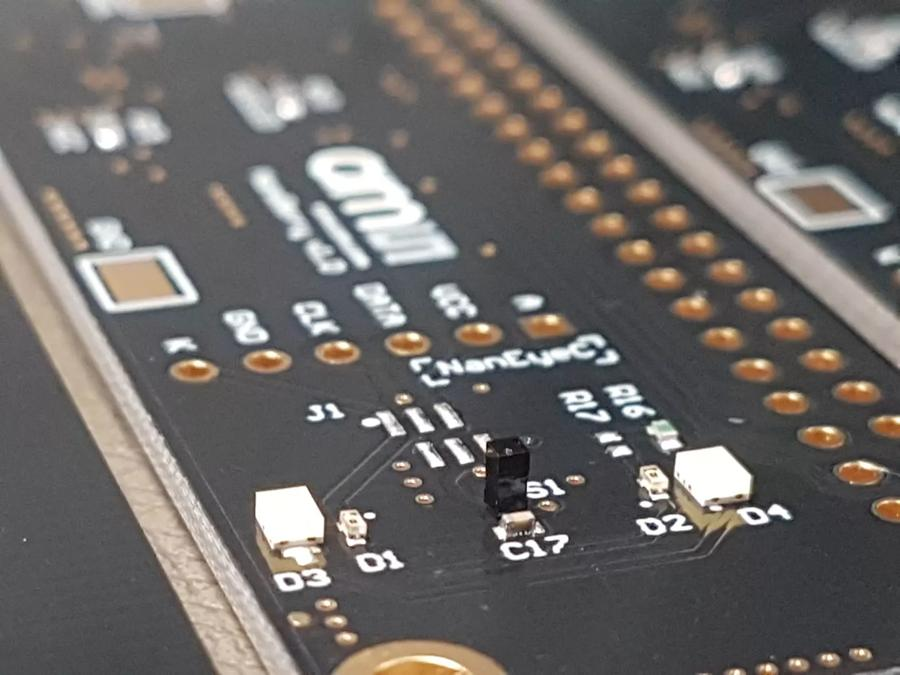
\includegraphics[width=\linewidth]{x01_nanoberry.jpg}\\[-2pt]{\small (a)}
\end{minipage}\hfill
\begin{minipage}[t]{0.56\linewidth}\centering
  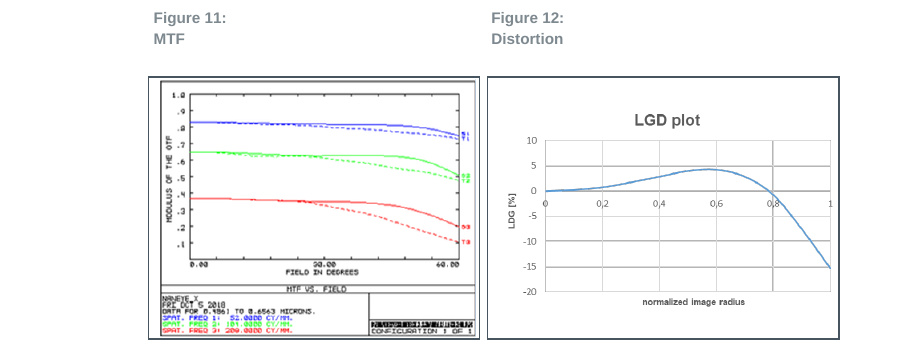
\includegraphics[width=\linewidth]{x02_mtf_crop.png}\\[-2pt]{\small (b)}
\end{minipage}
\caption{(a) Placa NanoBerry de ams: la NanEyeC es el cubo negro S1, con dos LED blancos. El conector J1 expone A, VCC, DATA, CLK, GND y K. Foto de la cámara, no tomada con ella~[S3]. (b) MTF y distorsión de la hoja de datos: la distorsión llega a $-15$\,\% en el borde del campo~[S1].}
\end{figure}

%=======================================================================
\section{Resolución esperada entre 5 y 12~mm}

El campo nominal se calculó con un modelo estenopeico: FOV diagonal de 120° y campo cuadrado de 320~px, sin distorsión (\texttt{calculo.py}).

\begin{table}[H]\centering
\caption{Campo y densidad de píxeles nominales, y valores medidos con la NanEyeM~[S7] (ejes de su Fig.~17).}
\small
\begin{tabular}{r r r r l}
\toprule
Distancia [mm] & Campo [mm] & px/mm & mm/px & Medido NanEyeM \\
\midrule
4  & 9,8  & 32,7 & 0,031 & 11,2~mm $\Rightarrow$ 28,6~px/mm \\
5  & 12,3 & 26,1 & 0,038 & -- \\
6  & 14,7 & 21,8 & 0,046 & 14,2~mm $\Rightarrow$ 22,5~px/mm \\
8  & 19,6 & 16,3 & 0,061 & -- \\
12 & 29,4 & 10,9 & 0,092 & -- \\
\bottomrule
\end{tabular}
\end{table}

Con 2 a 3~px por trazo, en el centro del campo se pueden separar detalles de $\approx$\,0,1~mm a 5~mm y de $\approx$\,0,25~mm a 12~mm. En los bordes es peor, por la distorsión y por la caída de luz. Es una estimación: hay que confirmarla con la prueba de la sección~\ref{sec:prueba}.

%=======================================================================
\section{Integración con la Kria K24}

\subsection{Modo de salida}
\begin{itemize}
  \item \textbf{SEIM (elegido).} Las señales son CMOS de 3,3~V. La FPGA genera SCLK (60--75~MHz) y el sensor devuelve SDAT sincronizado con ese reloj, con 2,1~ns de retardo. Entra en el banco HDIO~26 de la K24, que trabaja a 3,3~V y tiene 23 pines de usuario~[S5].
  \item \textbf{LVDS (descartado).} El reloj viaja embebido (Manchester). Además, la configuración se escribe a 3,3~V por los mismos pines, y los bancos HP de la K24 trabajan a 1,8~V como máximo.
\end{itemize}

\subsection{Qué hay que implementar}
\begin{itemize}
  \item \textbf{Placa:}
  \begin{itemize}
    \item footprint SGA de 4 pads, con perfil de reflujo a confirmar con el armador;
    \item LDO de 3,3~V dedicado, con capacitores de 220~nF o más junto al sensor;
    \item pistas cortas, con carga parásita menor a 5~pF y resistencia serie;
    \item iluminación propia (LED con PWM).
  \end{itemize}
  \item \textbf{FPGA:}
  \begin{itemize}
    \item reloj con MMCM y captura de SDAT con fase calibrada sobre el patrón de entrenamiento (los bancos HD no tienen IDELAY ni ISERDES);
    \item decodificación de las palabras de 12~bits: 8 palabras \texttt{010101010101} marcan el inicio de fila y 8 palabras nulas el fin de cuadro;
    \item salida AXI4-Stream con imagen RAW10 Bayer de 320\,$\times$\,320;
    \item escritura de configuración en la ventana de 648~PP: tramas de 24~bits (\texttt{1001} + dirección + 16~bits + \texttt{0}), y SDAT en alta impedancia después;
    \item demosaico y escritura a DDR.
  \end{itemize}
  \item \textbf{Linux:} driver V4L2 o UIO; exposición y balance de blancos por software; corrección de distorsión.
\end{itemize}

\subsection{Duración del cuadro}
Un cuadro tiene 648~PP de interfaz, 656 de sincronismo, el retardo mínimo de 656, 320 filas de 328~PP y 8~PP de fin de cuadro. Cada PP son 12 ciclos de SCLK~[S1].

El proyecto \emph{teensy\_naneyeC}~[S6] lee una NanEyeC del NanoBerry por SEIM con un microcontrolador, y sirve de control:
\begin{itemize}
  \item a 24,75~MHz su visor indica $\leq$\,19,3~cuadros/s, igual que el cálculo;
  \item a 12,375~MHz, con 258 filas de retardo, indica $\leq$\,5,4~cuadros/s, que es lo que da el mismo cálculo con ese retardo.
\end{itemize}

\begin{table}[H]\centering
\caption{Duración del cuadro en SEIM con el retardo mínimo (\texttt{calculo.py}).}
\small
\begin{tabular}{r r r}
\toprule
SCLK [MHz] & Cuadro [ms] & Cuadros/s \\
\midrule
12,375 & 103,7 & 9,6 \\
24,75  & 51,8  & 19,3 \\
60     & 21,4  & 46,8 \\
75     & 17,1  & 58,5 \\
\bottomrule
\end{tabular}
\end{table}

%=======================================================================
\section{Disponibilidad y proveedores}\label{sec:dispo}

\begin{table}[H]\centering
\caption{Situación de compra al 01/10/2026.}
\small
\begin{tabularx}{\linewidth}{l X}
\toprule
Ítem & Situación \\
\midrule
Fabricante & ams OSRAM, único. El ensamblado pasó a Focuslight (Singapur) en 2024; el contrato sigue siendo con ams~[S2]. \\
Códigos & RGB: Q65114A0180 (obsoleto) $\rightarrow$ \textbf{Q65113A9012}. Blanco y negro: Q65114A0181 $\rightarrow$ Q65113A9011~[S2]. \\
Estado & RGB en \emph{preproducción}; blanco y negro en producción plena~[S3]. \\
Sensor suelto & Solo bandeja de 496~u. DigiKey: USD~58,443 c/u, 0 en stock, 12 semanas~[S4]. \\
Kit NanoBerry color & DigiKey 14~u a USD~583,90; Mouser EU 3~u a EUR~450; Avnet 0~u, 56 semanas. \\
Distribuidores & DigiKey, Mouser, Arrow, Avnet, Rutronik, Future y Farnell. Para menos de 496~u: muestras de ams o bandeja parcial con el proyecto registrado. \\
NanEye2D & SGA solo en blanco y negro, sin lente, mínimo 400~u; RGB solo con cable de 2~m~[S26]. Descartada. \\
Alternativa & OMNIVISION OCHTA10 (Arrow 64~u, USD~72,16). Otra interfaz: necesita el puente OAH0428. \\
\bottomrule
\end{tabularx}
\end{table}

%=======================================================================
\section{Imágenes reales tomadas con cámaras NanEye}

\subsection{Criterio}
Se incluyen solo capturas que la fuente atribuye explícitamente a una cámara NanEye. Se dejaron afuera las fotos del módulo, los esquemas, los renders y las imágenes de otras cámaras. En figuras compuestas, el pie dice qué paneles son NanEye.

Hay tres generaciones distintas:
\begin{itemize}
  \item \textbf{NanEye 2D / 2C:} 250\,$\times$\,250~px, 3~$\mu$m;
  \item \textbf{NanEyeM:} 320\,$\times$\,320~px, el mismo sensor y la misma óptica que la NanEyeC;
  \item \textbf{NanEyeC:} la cámara evaluada.
\end{itemize}
Una captura de la NanEye 2D no demuestra el rendimiento de la NanEyeC. Cuando un dato no está publicado, se indica «no indicado».

\begin{table}[H]\centering
\caption{Resumen de las imágenes. Relevancia para leer etiquetas a 5--12~mm: A alta, M media, B baja.}
\scriptsize
\begin{tabularx}{\linewidth}{l l l l X c}
\toprule
Fig. & Fuente & Modelo & Lente & Distancia y objeto & Rel. \\
\midrule
\ref{fig:c01}--\ref{fig:c05} & [S6] & NanEyeC RGB & de fábrica & no indicada; escenas de laboratorio & M \\
\ref{fig:m01}--\ref{fig:m03} & [S7] & NanEyeM & de fábrica & 2--10~mm; tejido, MTF & A \\
\ref{fig:o05}--\ref{fig:o06} & [S16] & NanEyeM & no indicada & no indicada; columna & M \\
\ref{fig:r03} & [S9] & NanEye 250\,$\times$\,250 & ventana propia & contacto a 20~mm; carta USAF & A \\
\ref{fig:r01}--\ref{fig:r02} & [S8] & NanEye RGB & 90°, F2.7 & 8,0~mm; relieves de 1~mm & A \\
\ref{fig:r04}--\ref{fig:r05} & [S10,~S11] & NanEye 2C & no indicada & no indicada / 1--2~cm; texto & A \\
\ref{fig:r06}--\ref{fig:r07} & [S12] & NanEye & óptica propia & campo de 4~mm; USAF, piel & M \\
\ref{fig:r08} & [S13] & NanEye & no indicada & no indicada; cuadrícula & M \\
\ref{fig:o01}--\ref{fig:o04} & [S14,~S15] & NanEye 2D B/N & 90°, F2.7 & 13~mm / no indicada; speckle & B \\
\ref{fig:o07}--\ref{fig:o15} & varias & NanEye 2D, Stereo & varias & no indicada; tejido, ojo, sol & B \\
\bottomrule
\end{tabularx}
\end{table}

\subsection{NanEyeC en el kit NanoBerry}
Las Figs.~\ref{fig:c01} a \ref{fig:c05} son capturas de \emph{teensy\_naneyeC}~[S6]: la NanEyeC RGB del NanoBerry, leída por SEIM. No se indica la distancia; las escenas están a centímetros o metros. Sirven para ver el color, el ruido y la distorsión reales del sensor, no la lectura a 5--12~mm.

\fig{c01_teensy_color.png}{0.80}{NanEyeC RGB en el NanoBerry, imagen en color, a 12,375~MHz y 5,3~cuadros/s, con exposición de 184~ms y LED a 5~mA. Procesamiento básico: demosaico bilineal, balance \emph{grey world} y gamma 1,0~[S6].\label{fig:c01}}

\begin{figure}[H]\centering
\begin{minipage}[t]{0.55\linewidth}\centering
  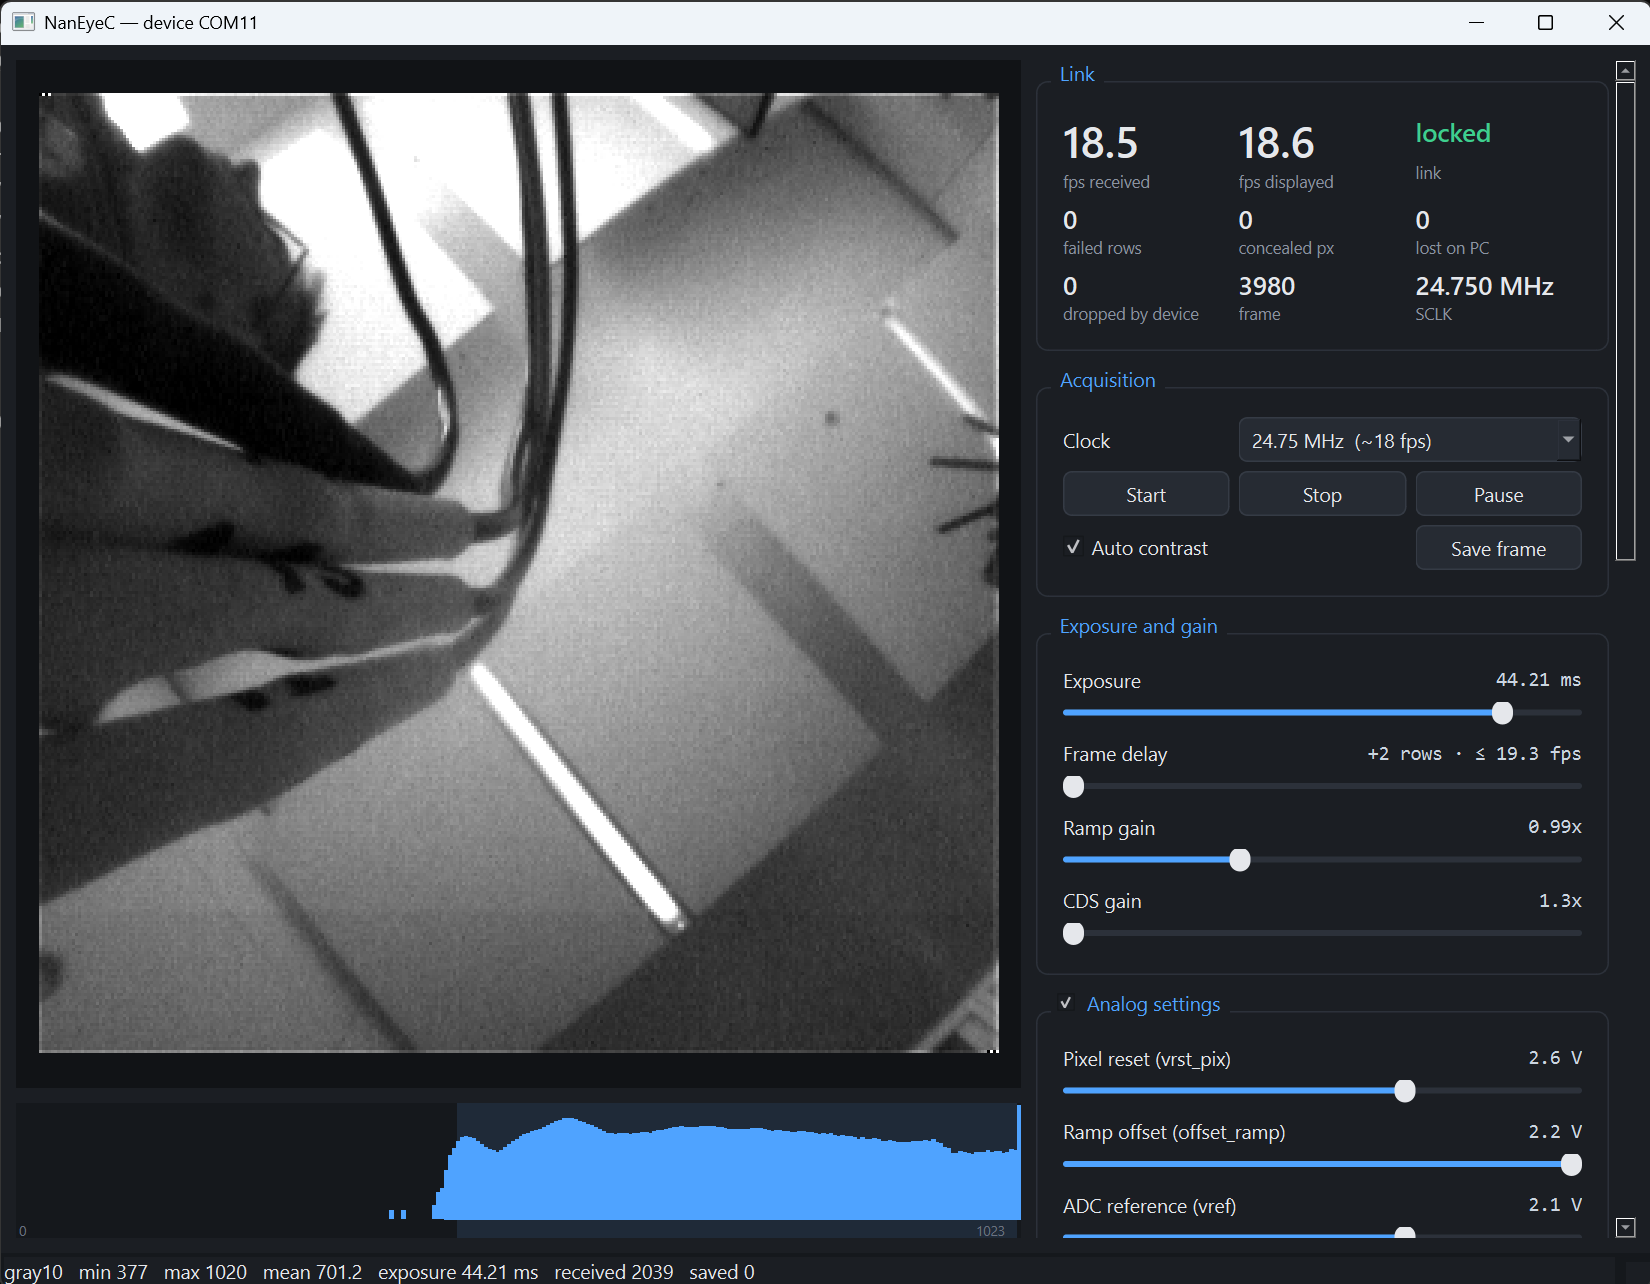
\includegraphics[width=\linewidth]{c02_teensy_gris.png}\\[-2pt]{\small (a)}
\end{minipage}\hfill
\begin{minipage}[t]{0.42\linewidth}\centering
  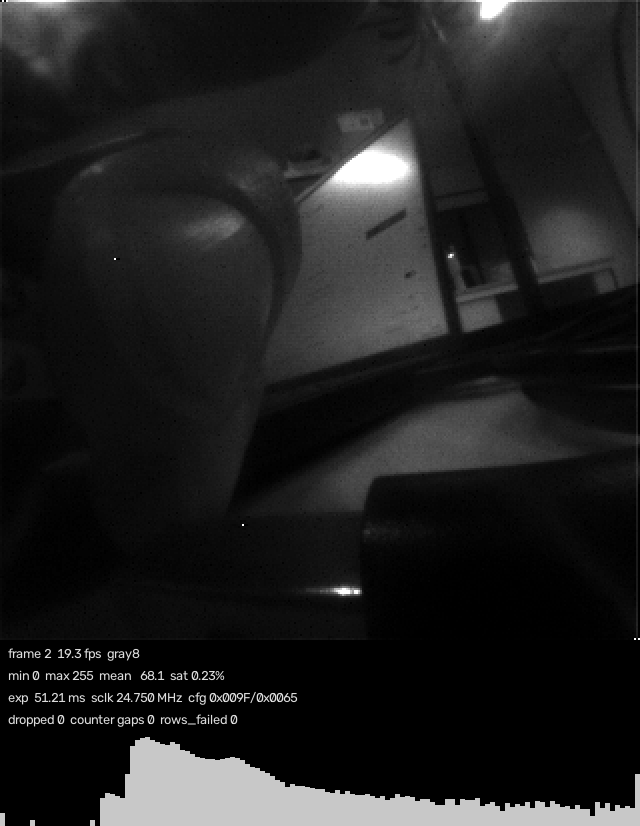
\includegraphics[width=\linewidth]{c04_teensy_pocaluz.png}\\[-2pt]{\small (b)}
\end{minipage}
\caption{NanEyeC, imagen en grises de 10 y 8~bits. (a) A 24,75~MHz y 18,5~cuadros/s, con exposición de 44~ms. (b) Con poca luz, exposición de 51~ms~[S6].\label{fig:c02}}
\end{figure}

\fig{c03_teensy_mano.png}{0.42}{NanEyeC, mano con cables a corta distancia (no indicada): se ven la distorsión de barril y la saturación junto al LED~[S6].\label{fig:c03}}

\fig{c05_teensy_led.png}{0.95}{NanEyeC, respuesta al LED del NanoBerry: nivel medio contra corriente (lineal, 1,98~DN/mA), imagen a 20~mA y diferencia con el LED apagado~[S6].\label{fig:c05}}

\subsection{NanEyeM (misma óptica que la NanEyeC)}
El endoscopio de 1,8~mm de [S7] usa la NanEyeM con un único micro-LED.

\fig{m01_naneyem_fig24.jpg}{0.85}{NanEyeM, trompa de Falopio de cerdo ex vivo, con ganancia fija, 120~ms de exposición y barra de escala de 3~mm. La distancia por imagen no está indicada; el ensayo se hizo a pocos mm~[S7, Fig.~24].\label{fig:m01}}

\fig{m02_naneyem_fig23.jpg}{0.95}{NanEyeM, aparato reproductor de cerdo ex vivo, con ganancia y exposición automáticas~[S7, Fig.~23].\label{fig:m02}}

\fig{m03_naneyem_mtf.jpg}{0.95}{NanEyeM, MTF medida con borde inclinado entre 2 y 10~mm: (a) ganancia automática; (b) ganancia fija. Es un gráfico obtenido de capturas de la cámara~[S7, Fig.~18].\label{fig:m03}}

\fig{o05_vine_fig3.jpg}{0.80}{NanEyeM en un robot de eversión, dentro de un modelo de columna. Solo la fila D es de la NanEyeM, en color; las demás son fotos externas y gráficos. Distancia no indicada~[S16, Fig.~3].\label{fig:o05}}

\fig{o06_vine_fig5.jpg}{0.70}{El mismo robot en un cadáver humano. Solo la fila E es de la NanEyeM; las demás son fluoroscopias y fotos externas~[S16, Fig.~5].\label{fig:o06}}

\subsection{Capturas cercanas de patrones, relieves y texto}

\fig{r03_patente_fig29.png}{0.78}{Carta USAF 1951 impresa a 1200~ppp, a contacto, 5, 10, 15 y 20~mm. \textbf{Solo las filas c y d son NanEye} (250\,$\times$\,250~px), detrás de las ventanas distal y lateral de un neuroendoscopio. Las filas a y b son un fibroscopio y la e un endoscopio rígido. La impresión en semitono degrada la imagen. El texto de la patente nombra esta figura como «Fig.~30»: es un error~[S9].\label{fig:r03}}

\fig{r01_micromach_fig5.jpg}{0.75}{NanEye RGB, FOV~90°, F2.7, a 8,0~mm de un modelo de tejido con relieves de 1,0~mm. (a)--(d) son capturas directas, cada una con una fibra de iluminación distinta; (e) es la reconstrucción procesada~[S8, Fig.~5].\label{fig:r01}}

\fig{r02_micromach_fig6.jpg}{0.55}{La misma cámara y montaje a 8~mm. \textbf{Solo la fila superior} («White 6500K Uncorrected») es captura directa; las demás están procesadas. Las columnas son la profundidad del objetivo bajo la superficie (0 a 2~mm), no la distancia a la cámara~[S8, Fig.~6].\label{fig:r02}}

\begin{figure}[H]\centering
\begin{minipage}[c]{0.30\linewidth}\centering
  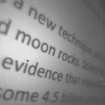
\includegraphics[width=\linewidth]{r04_handsight14_fig3.png}\\[-2pt]{\small (a)}
\end{minipage}\hfill
\begin{minipage}[c]{0.66\linewidth}\centering
  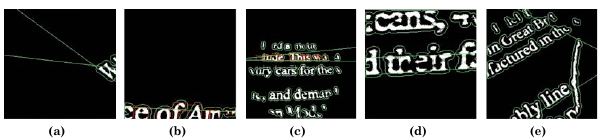
\includegraphics[width=\linewidth]{r05_handsight16_fig11.png}\\[-2pt]{\small (b)}
\end{minipage}
\caption{Texto impreso visto con una NanEye 2C (250\,$\times$\,250~px, con anillo de LED) montada en un anillo de dedo. (a) Captura cruda en grises; distancia no indicada~[S10, Fig.~3]. (b) Capturas preprocesadas: binarizadas y con líneas de base superpuestas. En ese estudio la cámara iba a 1--2~cm del papel, con un campo de $\approx$\,1,5~cm~[S11, Fig.~11].\label{fig:r04}\label{fig:r05}}
\end{figure}

\begin{figure}[H]\centering
\begin{minipage}[c]{0.56\linewidth}\centering
  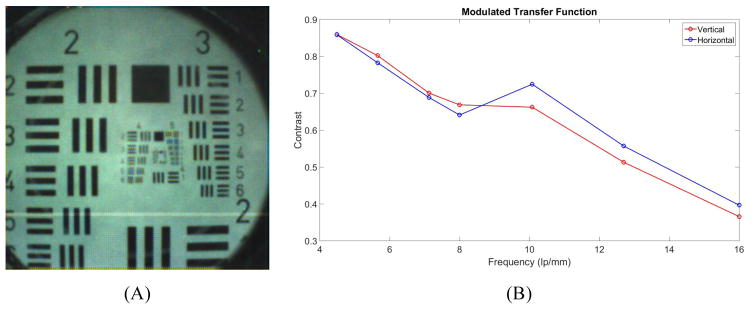
\includegraphics[width=\linewidth]{r06_dermo_usaf.jpg}\\[-2pt]{\small (a)}
\end{minipage}\hfill
\begin{minipage}[c]{0.40\linewidth}\centering
  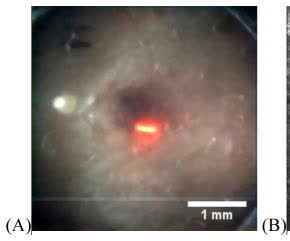
\includegraphics[width=\linewidth]{r07_dermo_piel_a.jpg}\\[-2pt]{\small (b)}
\end{minipage}
\caption{NanEye en color con \textbf{óptica propia} (hiperhemisferio de un objetivo de microscopio), con un campo de 4~mm. (a) Carta USAF 1951 y MTF medida (13~lp/mm al 50\,\%). (b) Lunar de piel, con barra de 1~mm. No representa la óptica de fábrica~[S12, Figs.~6 y 7A].\label{fig:r06}\label{fig:r07}}
\end{figure}

\fig{r08_edom_grilla.jpg}{0.60}{Cuadrícula fotografiada con una NanEye: lente multi-elemento de ams (izquierda) contra lente simple (derecha). La publica el distribuidor oficial EDOM; no indica modelo ni distancia~[S13].\label{fig:r08}}

\subsection{Otras capturas (relevancia baja)}

\begin{figure}[H]\centering
\begin{minipage}[t]{0.52\linewidth}\centering
  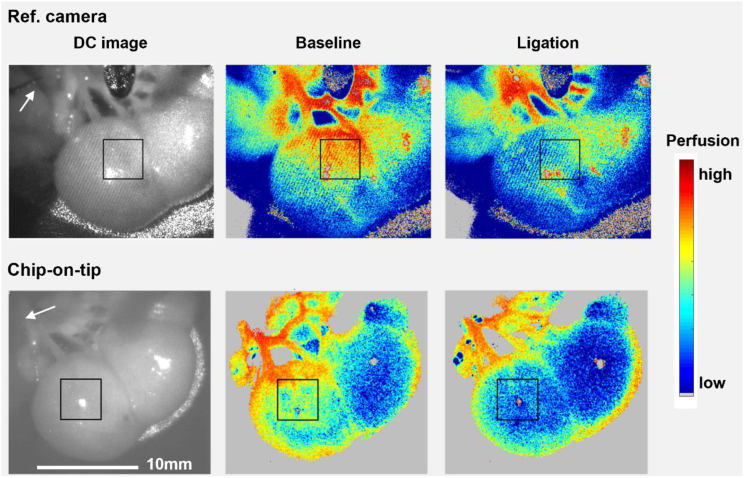
\includegraphics[width=\linewidth]{o01_lsci_fig3.jpg}\\[-2pt]{\small (a)}
\end{minipage}\hfill
\begin{minipage}[t]{0.44\linewidth}\centering
  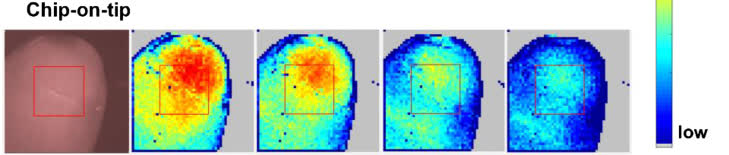
\includegraphics[width=\linewidth]{o03_lsci_fig4A.jpg}\\[-2pt]{\small (b)}
\end{minipage}
\caption{NE2D B/N FOV90 F2.7 a 13~mm, con láser de 785~nm. (a) Fila «Chip-on-tip», imagen DC de un feto de ratón con barra de 10~mm; los mapas de perfusión son procesados. (b) Fila «Chip-on-tip», yema de dedo: la imagen DC tiene el color agregado después y los mapas son procesados~[S14, Figs.~3 y 4].\label{fig:o01}\label{fig:o03}}
\end{figure}

\begin{figure}[H]\centering
\begin{minipage}[t]{0.40\linewidth}\centering
  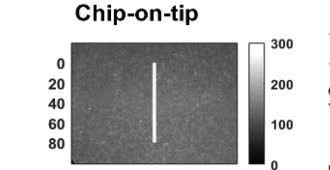
\includegraphics[width=\linewidth]{o02_lsci_fig2B.jpg}\\[-2pt]{\small (a)}
\end{minipage}\hfill
\begin{minipage}[t]{0.56\linewidth}\centering
  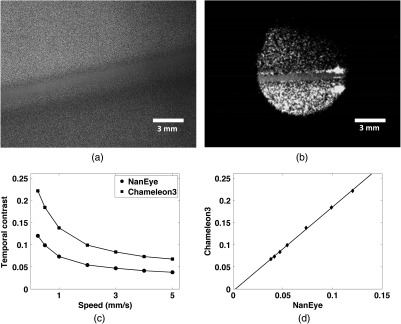
\includegraphics[width=\linewidth]{o04_encia_fig2.jpg}\\[-2pt]{\small (b)}
\end{minipage}
\caption{Speckle crudo de microcanales. (a) Panel «Chip-on-tip» de [S14, Fig.~2B], a 13~mm. (b) Panel (b), NanEye con lente f/2.7 (8--75~mm de profundidad de foco) dentro de una carcasa que recorta el campo; el panel (a) es otra cámara. Distancia no indicada~[S15, Fig.~2].\label{fig:o02}\label{fig:o04}}
\end{figure}

\begin{figure}[H]\centering
\begin{minipage}[t]{0.40\linewidth}\centering
  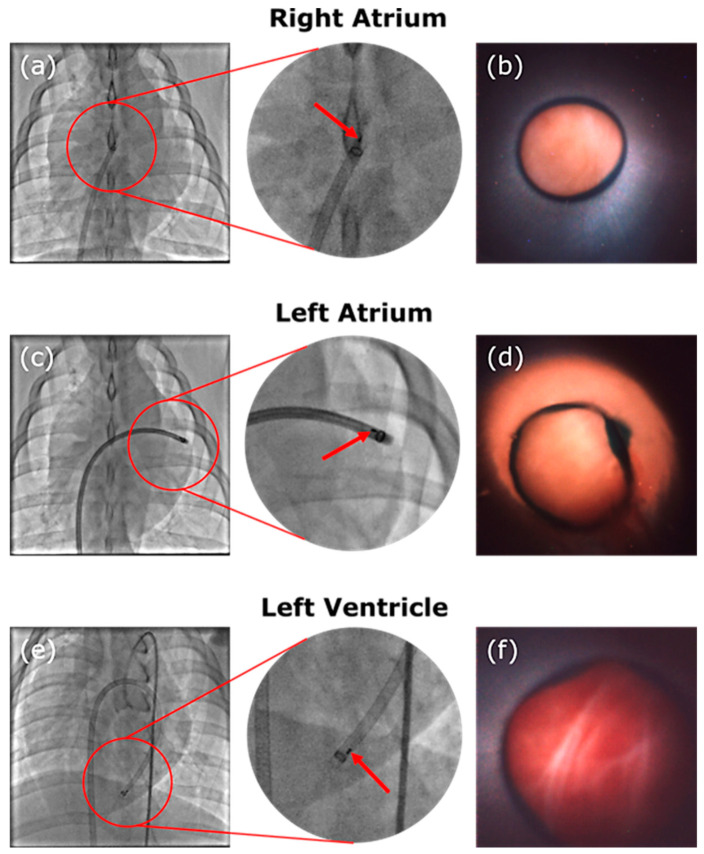
\includegraphics[width=\linewidth]{o07_cateter_fig6.jpg}\\[-2pt]{\small (a)}
\end{minipage}\hfill
\begin{minipage}[t]{0.56\linewidth}\centering
  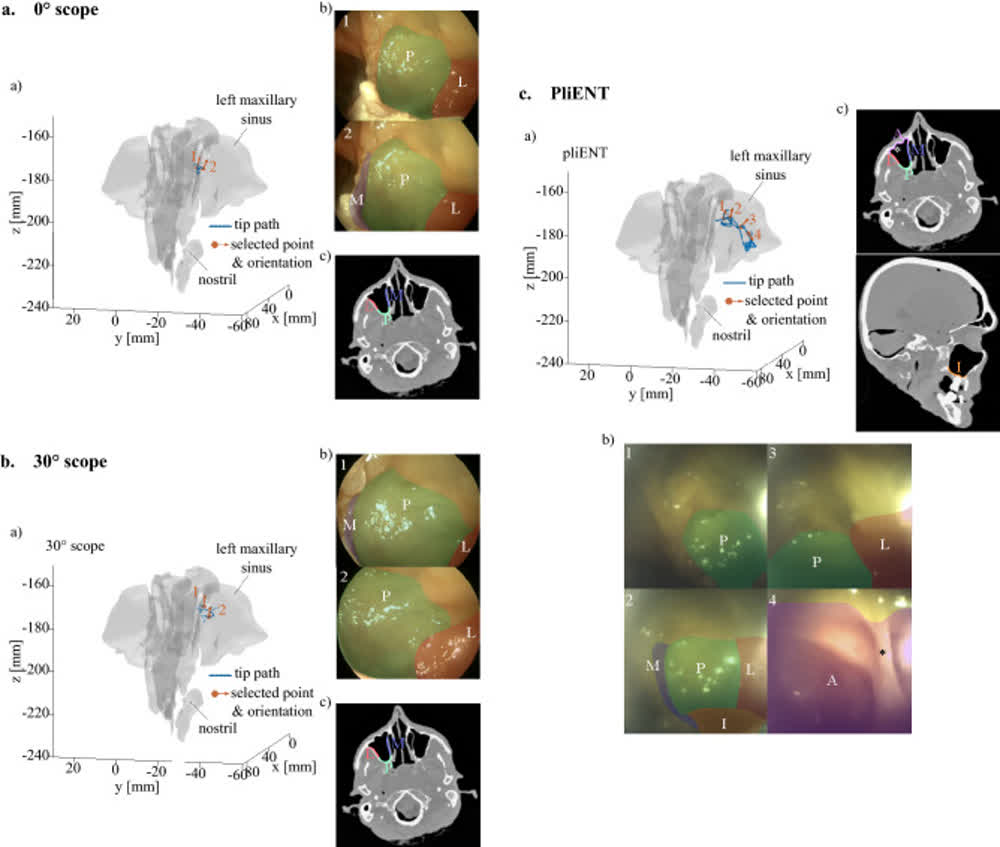
\includegraphics[width=\linewidth]{o08_pliENT_fig7.jpg}\\[-2pt]{\small (b)}
\end{minipage}
\caption{(a) NE2D RGB V120F2.8 en un corazón de cerdo in vivo: paneles b, d y f; los paneles a, c y e son fluoroscopias~[S17, Fig.~6]. (b) NanEye de 249\,$\times$\,250~px en el endoscopio PliENT, seno maxilar de cadáver: bloque c), paneles b)1--4, con segmentación superpuesta~[S18, Fig.~7]. Distancias no indicadas.\label{fig:o07}\label{fig:o08}}
\end{figure}

\begin{figure}[H]\centering
\begin{minipage}[b]{0.70\linewidth}\centering
  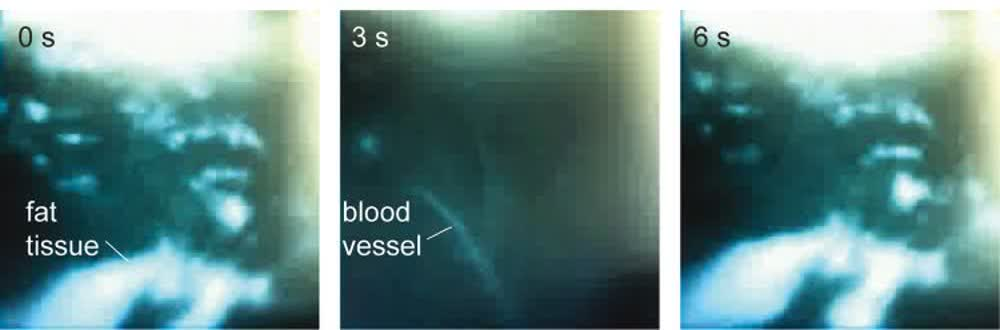
\includegraphics[height=3.6cm]{o09_cisto_fig6b.jpg}\\[-2pt]{\small (a)}
\end{minipage}\hfill
\begin{minipage}[b]{0.26\linewidth}\centering
  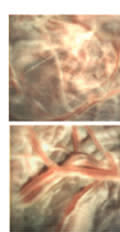
\includegraphics[height=3.8cm]{o10_feto_fig7a.jpg}\\[-2pt]{\small (b)}
\end{minipage}
\caption{(a) NanEye 2D en una vejiga de conejo, cuadros de video a 0, 3 y 6~s (fila b de la figura original)~[S19, Fig.~6b]. (b) NanEye Stereo, canal izquierdo, placenta humana ex vivo (panel a, dos cuadros)~[S20, Fig.~7a]. Distancias no indicadas.\label{fig:o09}\label{fig:o10}}
\end{figure}

\begin{figure}[H]\centering
\begin{minipage}[t]{0.32\linewidth}\centering
  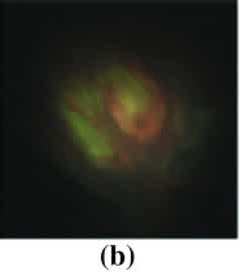
\includegraphics[width=\linewidth]{o11_placenta_fig6b.jpg}\\[-2pt]{\small (a)}
\end{minipage}\hfill
\begin{minipage}[t]{0.64\linewidth}\centering
  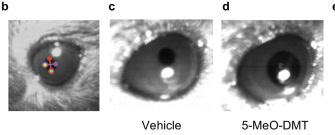
\includegraphics[width=\linewidth]{o12_oculometro_bcd.jpg}\\[-2pt]{\small (b)}
\end{minipage}
\caption{(a) NanEye en un fetoscopio flexible, placenta de silicona en agua (panel b de la figura original)~[S21, Fig.~6b]. (b) NE2D B/N V90F2.7, ojo de ratón con LED de 720~nm (paneles b, c y d); en b los puntos están marcados a mano~[S22, Fig.~4]. Distancias no indicadas.\label{fig:o11}\label{fig:o12}}
\end{figure}

\begin{figure}[H]\centering
\begin{minipage}[t]{0.30\linewidth}\centering
  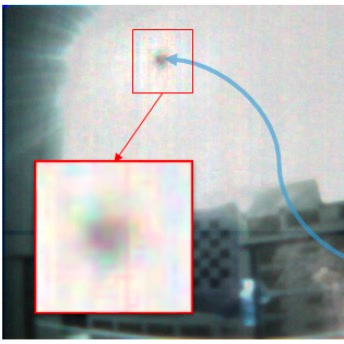
\includegraphics[width=\linewidth]{o13_sol_izq.jpg}\\[-2pt]{\small (a)}
\end{minipage}\hfill
\begin{minipage}[t]{0.22\linewidth}\centering
  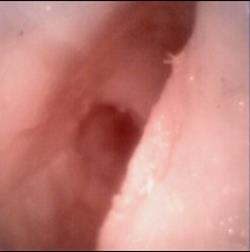
\includegraphics[width=\linewidth]{o14_pulmon.png}\\[-2pt]{\small (b)}
\end{minipage}\hfill
\begin{minipage}[t]{0.44\linewidth}\centering
  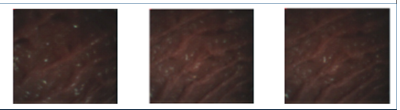
\includegraphics[width=\linewidth]{o15_capsula_naneye.png}\\[-2pt]{\small (c)}
\end{minipage}
\caption{(a) NanEye 2D apuntada al sol: saturación y «sol negro»~[S23, Fig.~1]. (b) NanEye 2D dentro de un pulmón, imagen nativa de 250\,$\times$\,252~px sin escalar~[S24, Fig.~3]. (c) Awaiba NanEye en un simulador de estómago (fila de la NanEye de la figura original; las otras filas son cámaras de inspección)~[S25, Fig.~1]. Distancias no indicadas.\label{fig:o13}\label{fig:o14}\label{fig:o15}}
\end{figure}

%=======================================================================
\section{Lectura de las imágenes}
\begin{itemize}
  \item \textbf{Nitidez:} pareja entre 4 y 10~mm (Fig.~\ref{fig:m03}). Las Figs.~\ref{fig:m01} y \ref{fig:r01} muestran detalle fino en el centro: pliegues de tejido y bordes de relieves de 1~mm a 8~mm.
  \item \textbf{Iluminación:} es la limitación más visible. Con una sola fuente puntual, la luz cae mucho hacia el borde (Figs.~\ref{fig:r01}, \ref{fig:r04} y \ref{fig:c05}) y aparecen reflejos que saturan píxeles (Fig.~\ref{fig:r02}, fila superior).
  \item \textbf{Distorsión:} de barril, visible en las Figs.~\ref{fig:c03} y \ref{fig:r08}. Hay que corregirla por software antes de medir o decodificar códigos.
  \item \textbf{Texto:} la Fig.~\ref{fig:r04}a, con una NanEye 2C de menos píxeles, se lee bien en el centro con letras de cuerpo normal y se vuelve ilegible hacia el borde. Con la NanEyeC a 5--8~mm la densidad es mayor (16--26~px/mm), pero no hay captura que lo confirme.
  \item \textbf{Color:} correcto pero apagado con el procesamiento básico (Fig.~\ref{fig:c01}). Necesita corrección de color y balance de blancos.
\end{itemize}

\textbf{Limitaciones de esta evidencia}
\begin{itemize}
  \item \textbf{Generación:} las capturas más cercanas y con patrones (Figs.~\ref{fig:r03}, \ref{fig:r04}, \ref{fig:r06}) son de la NanEye 2D/2C de 250\,$\times$\,250~px, no de la NanEyeC.
  \item \textbf{Óptica:} varias usan óptica propia o ventanas delante de la cámara (Figs.~\ref{fig:r03}, \ref{fig:r06}).
  \item \textbf{Reproducción:} las imágenes salen de PDFs, comprimidas y reescaladas; la patente está impresa en semitono.
  \item \textbf{Distancia:} solo las Figs.~\ref{fig:m03}, \ref{fig:r03}, \ref{fig:r01}, \ref{fig:r02} y \ref{fig:o01} la publican.
\end{itemize}

%=======================================================================
\section{Recomendación y prueba propuesta}\label{sec:prueba}
\begin{itemize}
  \item \textbf{Comprar un kit NanoBerry color} y montar la NanEyeC en un soporte con tornillo micrométrico.
  \item \textbf{Objetivos}, impresos a 1200~ppp o más:
  \begin{itemize}
    \item carta USAF 1951 y borde inclinado;
    \item texto de 4, 6 y 8~pt;
    \item QR y DataMatrix con módulos de 0,2, 0,3 y 0,5~mm;
    \item una etiqueta real.
  \end{itemize}
  \item \textbf{Distancias:} 5, 8 y 12~mm, con la iluminación final del robot y además con luz difusa. Exposición y ganancia fijas; guardar el RAW10 sin reescalar.
  \item \textbf{Medidas:}
  \begin{itemize}
    \item MTF50 en el centro y en el borde;
    \item último grupo USAF resuelto;
    \item tasa de decodificación de códigos (por ejemplo, con zxing);
    \item legibilidad del texto.
  \end{itemize}
  \item \textbf{En paralelo:}
  \begin{itemize}
    \item pedirle a ams muestras del Q65113A9012, la fecha de producción plena, una carta de ciclo de vida y el perfil de reflujo;
    \item hacer un adaptador del J1 del NanoBerry a pines HDIO para desarrollar el receptor SEIM en la K24.
  \end{itemize}
\end{itemize}

%=======================================================================
\section*{Fuentes}
\begin{small}
\begin{enumerate}[label={[S\arabic*]}, leftmargin=2.6em, itemsep=1pt]
  \item ams OSRAM, \emph{NanEyeC Miniature Camera Module}, DS000503 v2-00, 2022. \url{https://www.farnell.com/datasheets/4092303.pdf}
  \item ams OSRAM, Infonote AO-IN-2024-058-I, \emph{Transfer of OC production to Focuslight}, 15/09/2024. \url{https://mm.digikey.com/Volume0/opasdata/d220001/medias/docus/6403/AO-IN-2024-058-I_ext.pdf}
  \item ams OSRAM, página de producto NanEyeC y kit NanoBerry. \url{https://ams-osram.com/products/sensor-solutions/cmos-image-sensors/ams-naneyec-integrated-camera-module}
  \item DigiKey, NEC-HLBX-00-MODULE, consultado el 01/10/2026. \url{https://www.digikey.com/en/products/detail/ams-osram-usa-inc/NEC-HLBX-00-MODULE/25701847}
  \item AMD, \emph{Kria K24 SOM Data Sheet} (DS985). \url{https://www.mouser.com/pdfDocs/ds985-k24-som.pdf}
  \item phili-b, \emph{teensy\_naneyeC}, GitHub. \url{https://github.com/phili-b/teensy_naneyeC}
  \item \emph{A 1.8 mm-Diameter Chip-on-Tip Endoscope with Integrated $\mu$LED Illumination}, Sensors, 2026. \url{https://pmc.ncbi.nlm.nih.gov/articles/PMC13417079/}
  \item \emph{Microcamera Visualisation System to Overcome Specular Reflections for Tissue Imaging}, Micromachines 14:1062, 2023. \url{https://pmc.ncbi.nlm.nih.gov/articles/PMC10221823/}
  \item Patente US11464401B2 (familia EP3310243A1), neuroendoscopio multipuerto, Fig.~29. \url{https://patentimages.storage.googleapis.com/cb/09/cd/f4b13f70e0ef1a/US11464401.pdf}
  \item L.~Stearns et al., \emph{The Design and Preliminary Evaluation of a Finger-Mounted Camera\ldots}, ECCV-W ACVR, 2014. \url{https://makeabilitylab.cs.washington.edu/media/publications/Stearns_TheDesignAndPreliminaryEvaluationOfAFingerMountedCameraAndFeedbackSystemToEnableReadingOfPrintedTextForTheBlind_ACVR2014.pdf}
  \item L.~Stearns et al., \emph{Evaluating Haptic and Auditory Directional Guidance\ldots}, ACM TACCESS, 2016. \url{https://duruofei.com/papers/Stearns_EvaluatingHapticAndAuditoryDirectionalGuidanceToAssistBlindPeopleInReadingPrintedTextUsingFinger-MountedCameras_TACCESS2016.pdf}
  \item \emph{Dermoscopy-guided reflectance confocal microscopy of skin\ldots}, 2017. \url{https://pmc.ncbi.nlm.nih.gov/articles/PMC5597433/}
  \item EDOM Technology, \emph{NanEye: the smallest digital camera module has a huge vision}. \url{https://www.edomtech.com/en/article-detail/naneye-the-smallest-digital-camera-module-has-a-huge-vision/}
  \item \emph{In vivo laser speckle contrast imaging\ldots using a chip-on-tip camera}, iScience, 2024. \url{https://pmc.ncbi.nlm.nih.gov/articles/PMC10875563/}
  \item C.~Regan et al., \emph{Design and evaluation of a miniature laser speckle imaging device to assess gingival health}, JBO 21(10), 2016. \url{https://pmc.ncbi.nlm.nih.gov/articles/PMC5081569/}
  \item \emph{Eversion-based robots can enable safe access, steering and endoscopic imaging within the spinal subarachnoid space}, arXiv:2607.19274, 2026. \url{https://arxiv.org/abs/2607.19274}
  \item \emph{Design and Assembly of a Miniature Catheter Imaging System for In Vivo Heart Endoscopic Imaging}, Sensors 24:6216, 2024. \url{https://pmc.ncbi.nlm.nih.gov/articles/PMC11478442/}
  \item \emph{A miniature robotic steerable endoscope for maxillary sinus surgery called PliENT}, Sci.~Rep., 2022. \url{https://pmc.ncbi.nlm.nih.gov/articles/PMC8831515/}
  \item \emph{Wireless Acoustic-Surface Actuators for Miniaturized Endoscopes}, ACS AMI, 2017. \url{https://pmc.ncbi.nlm.nih.gov/articles/PMC5730945/}
  \item \emph{A Continuum Robot and Control Interface for Surgical Assist in Fetoscopic Interventions}, 2017. \url{https://pmc.ncbi.nlm.nih.gov/articles/PMC5495161/}
  \item \emph{Deep learning-based monocular placental pose estimation}, IJCARS, 2020. \url{https://pmc.ncbi.nlm.nih.gov/articles/PMC7419456/}
  \item \emph{Vigilance state dissociation induced by 5-MeO-DMT in mice}, Commun.~Biol., 2025. \url{https://pmc.ncbi.nlm.nih.gov/articles/PMC12873260/}
  \item \emph{Accurate and Cost-Effective Micro Sun Sensor based on CMOS Black Sun Effect}, Sensors, 2019. \url{https://pmc.ncbi.nlm.nih.gov/articles/PMC6386896/}
  \item Awaiba, \emph{Miniature Camera Modules for Visualizing Micro Invasive Surgery} (white paper). \url{https://www.ushio.com/files/white-papers/nathaniel/awaiba-miniature-camera-modules-for-visualizing-micro-invasive-surgery.pdf}
  \item M.~Turan et al., arXiv:1705.06524, 2017. \url{https://arxiv.org/pdf/1705.06524}
  \item ams OSRAM, \emph{NanEye2D Miniature Camera Module}, DS000501 v10-00, 2024. \url{https://look.ams-osram.com/m/7cc9c2831b1d4049/original/NanEye-Miniature-Camera-Module-NanEye2D.pdf}
\end{enumerate}
\end{small}

\end{document}
